\documentclass[twocolumn,letterpaper,10pt]{article}
\usepackage{iasted}
\usepackage{times}
\usepackage{graphicx}
\usepackage{gensymb}
\begin{document}

\title{A New Sign Detection and Tracking Method for Intelligent Vehicles}

%  \author{
%  First A. Author \\
%  Department or Laboratory\\
%  University or Company\\
%  Address, (if necessary) \\
%  City, Province or State, Country \\
%  email: email-address \\
%  \and
%  Second B. Author and Third C. Author\\
%  Department or Laboratory\\
%  University or Company\\
%  Address (if necessary)\\
%  City, Province or State, Country \\
%  email: email-address \\
%  }

\maketitle
\thispagestyle{empty}


\begin{abstract}
Traffic signs are one of the most important instruments to indicate the rules on roads. It is clear that leaving traffic signs out of account will cause serious consequences in autonomous urban driving. Although the car manufacturers have started to deploy intelligent sign detection systems on their new models, the conditions and variations of actual signs on the roads require more robust and fast detection and tracking methods. In this paper a fast and robust sign detection and tracking method based on geometric transformation and genetic algorithms (GA) is presented. The GA output is filtered with a radial symmetry check so that false alerts are considerably reduced.  %Final paper'da (olursa) açılacak: This work is a part of the ADES (Automatic Driver Evaluation System) Project in Artificial Intelligence Laboratory of Bo{\u g}azi{\c c}i University. 
\\~\\{\bf Keywords:} Computer Vision, Traffic Sign Detection, Geometric Transformation, Genetic Algorithms, Radial Symmetry Check\\~
\end{abstract}

\section{Introduction}

Traffic accidents are one of the main causes of death and economic loss in most of the developed countries. According to the Road Safety Action Program of European Commission, more than one million accidents a year cause more than 40 000 deaths and nearly two million injuries on the roads. In addition, the direct and indirect cost has been estimated at 160 billion Euros, which is nearly two percent of the EU's GNP ~\cite{Eu01}. However, the most regretful fact is that, nearly all of the accidents are caused by driver mistakes. The main goal of the driver assistance and early warning systems are reducing the number of these accidents. However, the performance of such systems depend on their power to recognize the conditions and rules in the vehicle's existing context. Moreover, since most of the rules are expressed by traffic signs, robust and fast sign detection methods are inevitable for intelligent vehicles.


There are numerous methods for the detection and recognition of traffic signs. Escalera et. al. used color thresholding and shape analysis for detection, and neural networks for recognition ~\cite{Delaescalera97}. Fang et al. developed a neural network based approach for detection and a Kalman Filter for tracking the signs ~\cite{Fang03}. Hsu et al. proposed a template matching based for detection and matching pursuit filters, which decompose patterns into  two dimensional wavelet expansions for recognition ~\cite{Hsu01}. Bahlmann et al. used Haar wavelet features obtained from Ada-Boost training for detection and LDA followed by maximum likelihood approach for recognition ~\cite{Bahlmann05}. Loy et al. modified radial symmetry transform for detection ~\cite{Loy04}. Bascon et al. used shape classification using linear SVMs for detection and Gaussian-kernel SVMs for recognition ~\cite{Maldonadobascon07}. Escalera et. al. and Soetedjo et al. proposed  GA based methods for sign detection ~\cite{Delaescalera03}. Gao et al. uses shape and color based feature extraction methods for recognizing signs ~\cite{Gao06}. Similarly, H. Fleyeh proposed a fuzzy approach for color detection and segmentation of traffic signs ~\cite{Fleyeh05}.


This study is a part of an ongoing project called Automatic Driver Evaluation System (ADES). The proposed approach encodes the genetic algorithms (GA) chromosomes by using the geometric transformation matrix. The fitness function is calculated by using a set of transformed points which corresponds to the shape of the traffic signs. A radial symmetry test is performed to eliminate the false alerts.

The organization of the rest of the paper is as follows. In section \ref{sec:pa} we describe the proposed approach. A modified radial symmetry application for eleminating false pozitive results is introduced in the following section. In section \ref{sec:er} experimental results are presented. And finally in last section the conclusions and discussion points are given.

\section{Proposed Approach}
\label{sec:pa}
The proposed approach for sign detection and tracking in the ADES project is based on GA. A modified version of radial symmetric transform is applied after an image binarization. 
\subsection{Image Binarization}
The binarization method, given in Equation \ref{eq4}, is a function of red, green, and blue channels instead of a fixed color map.
\begin{eqnarray}
\label{eq4}
\nonumber f(r,g,b)&=& \left\{\begin{array}{l} 1 \rightarrow r>\alpha.g, r>\beta.b \\ 0 \rightarrow o/w \end{array}\right\}\\
\alpha &<& 1 \\
\nonumber \beta &<& 1
\end{eqnarray}
\par
\noindent The performance of the method highly depends on the proper calculation of $\alpha$ and $\beta$ coefficients. The proposed approach updates these coefficients with a specific period according to the histogram calculations of the current frame. Sample scenes with corresponding red, green, blue histograms, and their means and standard deviations of these histogram values are given in Figure \ref{fig:hist1} and  \ref{fig:hist2}.
\begin{figure}[ht]
\begin{center}
\includegraphics[width=80mm,height=90mm]{img/hist1.eps}
\caption{Good, medium and poor conditions for traffic sign detection.}
\label{fig:hist1}
\end{center}
\end{figure}
\par
\begin{figure}[ht]
\begin{center}
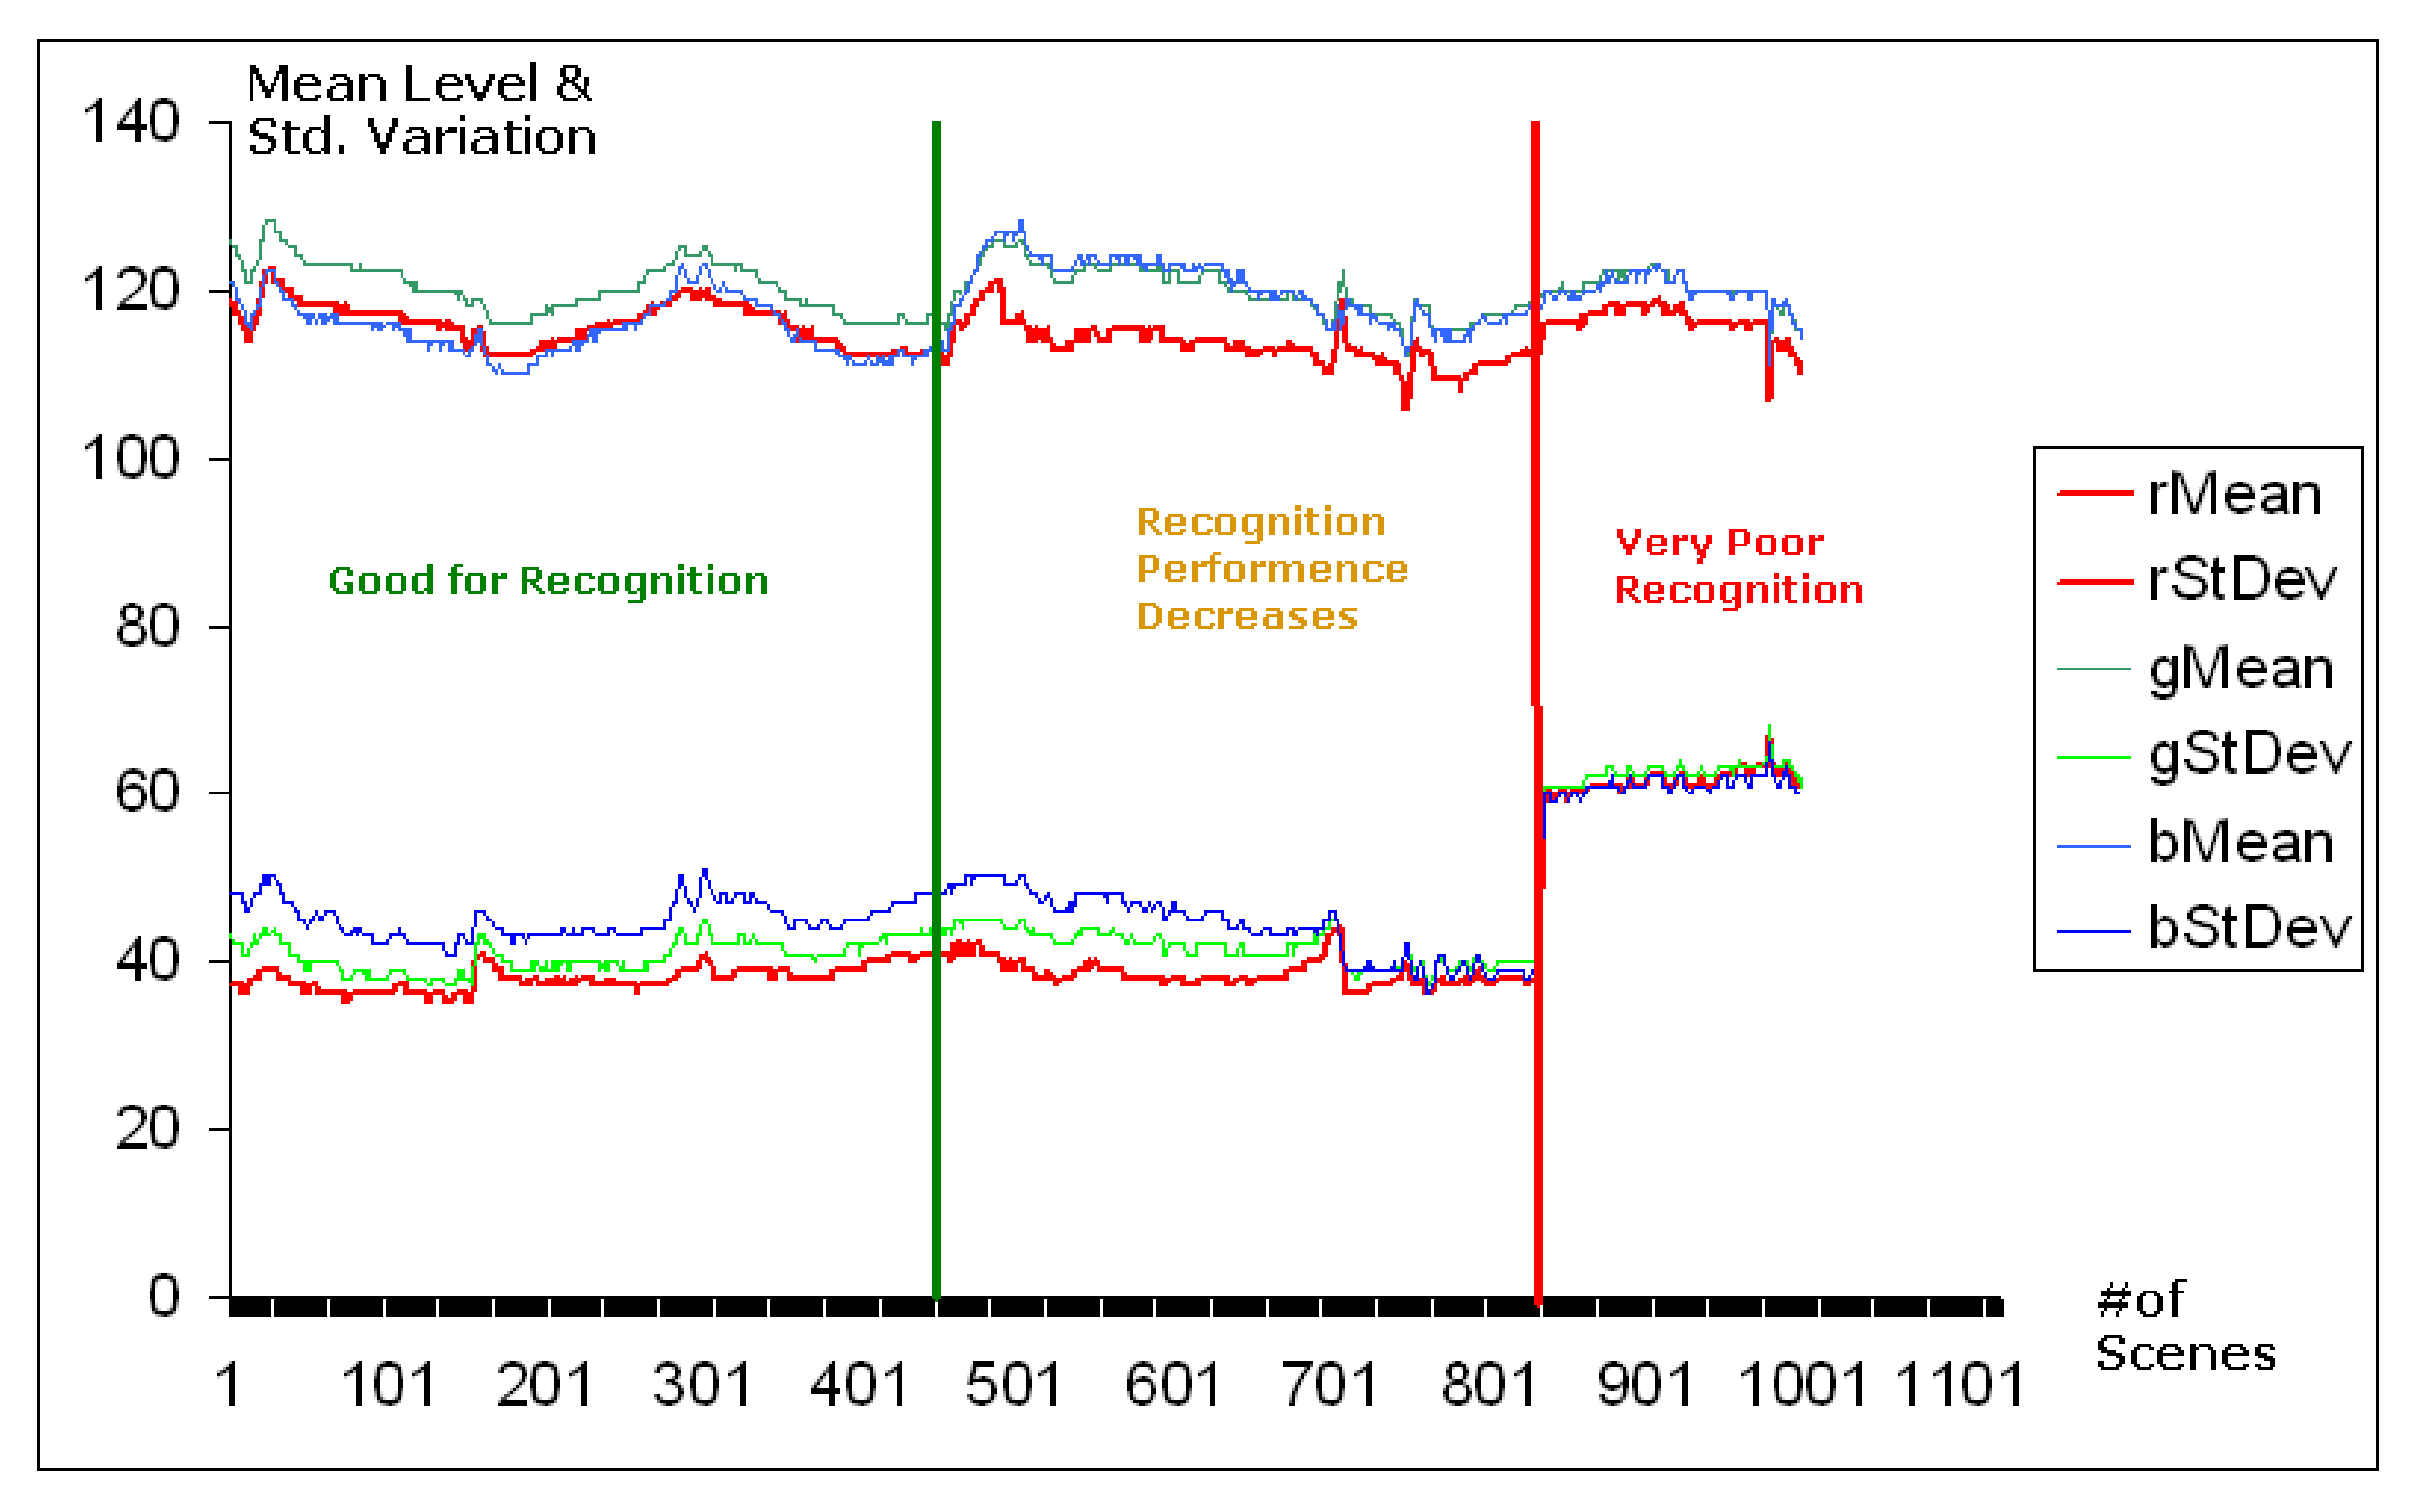
\includegraphics[width=70mm,height=50mm]{img/hist2.eps}
\caption{Means and standard deviations of sample scene histograms.}
\label{fig:hist2}
\end{center}
\end{figure}
\begin{eqnarray}
\label{eq42}
\nonumber STD_{all} &=& ((R_{StDev} + G_{StDev} + B_{StDev})/3)/128 \\
\nonumber RG_{mean} &=& (R_{mean}-G_{mean})/\sqrt{128} \\
RB_{mean} &=& (R_{mean}-B_{mean})/\sqrt{128} \\
\nonumber \alpha &=& 1 - 1 / (128 \times RG_{mean} \times STD_{all}) \\
\nonumber \beta &=& 1 - 1 / (128 \times RB_{mean} \times STD_{all})
\end{eqnarray}
\par
The values of $\alpha$ and $\beta$ coefficients are calculated according to Equation \ref{eq42} where $R$, $G$, and $B$ denote the red, green, and blue histogram arrays. Using histogram values for updating color remapping coefficients instead of applying adaptive histogram equalization improves the performance of the system. The original image and the produced binary image is given in Figure \ref{fig:sdfig1}.
\begin{figure}[ht]
\begin{center}
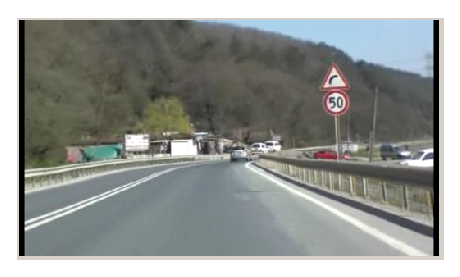
\includegraphics[width=70mm,height=40mm]{img/sdfig1.eps}
\includegraphics[width=70mm,height=40mm]{img/sdfig2.eps}
\caption{Original and binarized images.}
\label{fig:sdfig1}
\end{center}
\end{figure}
\subsection{GA Methodology}
The GA implementation uses the coefficients of a geometric transformation applied to a set of points which describes the characteristics of any searched template. The geometric transformation, which includes affine and perspective transformations, is
\begin{eqnarray}
\label{eq2}
\left| \begin{array}{ccc} u' \\ v' \\ w \end{array} \right| &=& 
\left| \begin{array}{ccc} a & b & c \\ d & e & f \\ g & h & 1 \end{array} \right| \left| \begin{array}{ccc} x \\ y \\ 1 \end{array} \right| \\
u &=& u'/w \\
v &=& v'/w 
\end{eqnarray}
\noindent where $x$ and $y$ are the coordinates of the sample point from the template describing the set of points. $u$ and $v$ are the transformed points on the image. $a$, $b$, $d$, $e$  provide rotation, scaling and shearing where $c$ and $f$ are used for translation. In addition, $g$ and $h$ provide perspective transformation in two dimensions. These coefficient values or a subset of them can be used in the chromosome encoding of the GA.

The effect of the transformation can be visualized better with a simple example. Assume that $a$, $b$, $c$, $d$, $e$, and $f$ coefficients are used in the encoding of the GA chromosome. In addition, $g$ and $h$ are left zero for simplicity. For this scenario, we can conclude that a chromosome with the transformation coefficients in Equation \ref{eq3} can yield the transformed circle and triangular points shown in Figure \ref{fig:sdfig2}. The points on the left hand side of each figure are the equidistant characteristic points of the circular and triangular templates, where the points on the right hand sides are the translated, scaled, and rotated counter parties in the transformed domain. 
\begin{eqnarray}
\label{eq3}
\left| \begin{array}{ccc} u \\ v \\ 1 \end{array} \right| &=& 
\left| \begin{array}{ccc} 2 & 1 & 100 \\ 1 & 2 & 50 \\ 0 & 0 & 1 \end{array} \right| \left| \begin{array}{ccc} x \\ y \\ 1 \end{array} \right|
\end{eqnarray}
\begin{figure}[ht]
\begin{center}
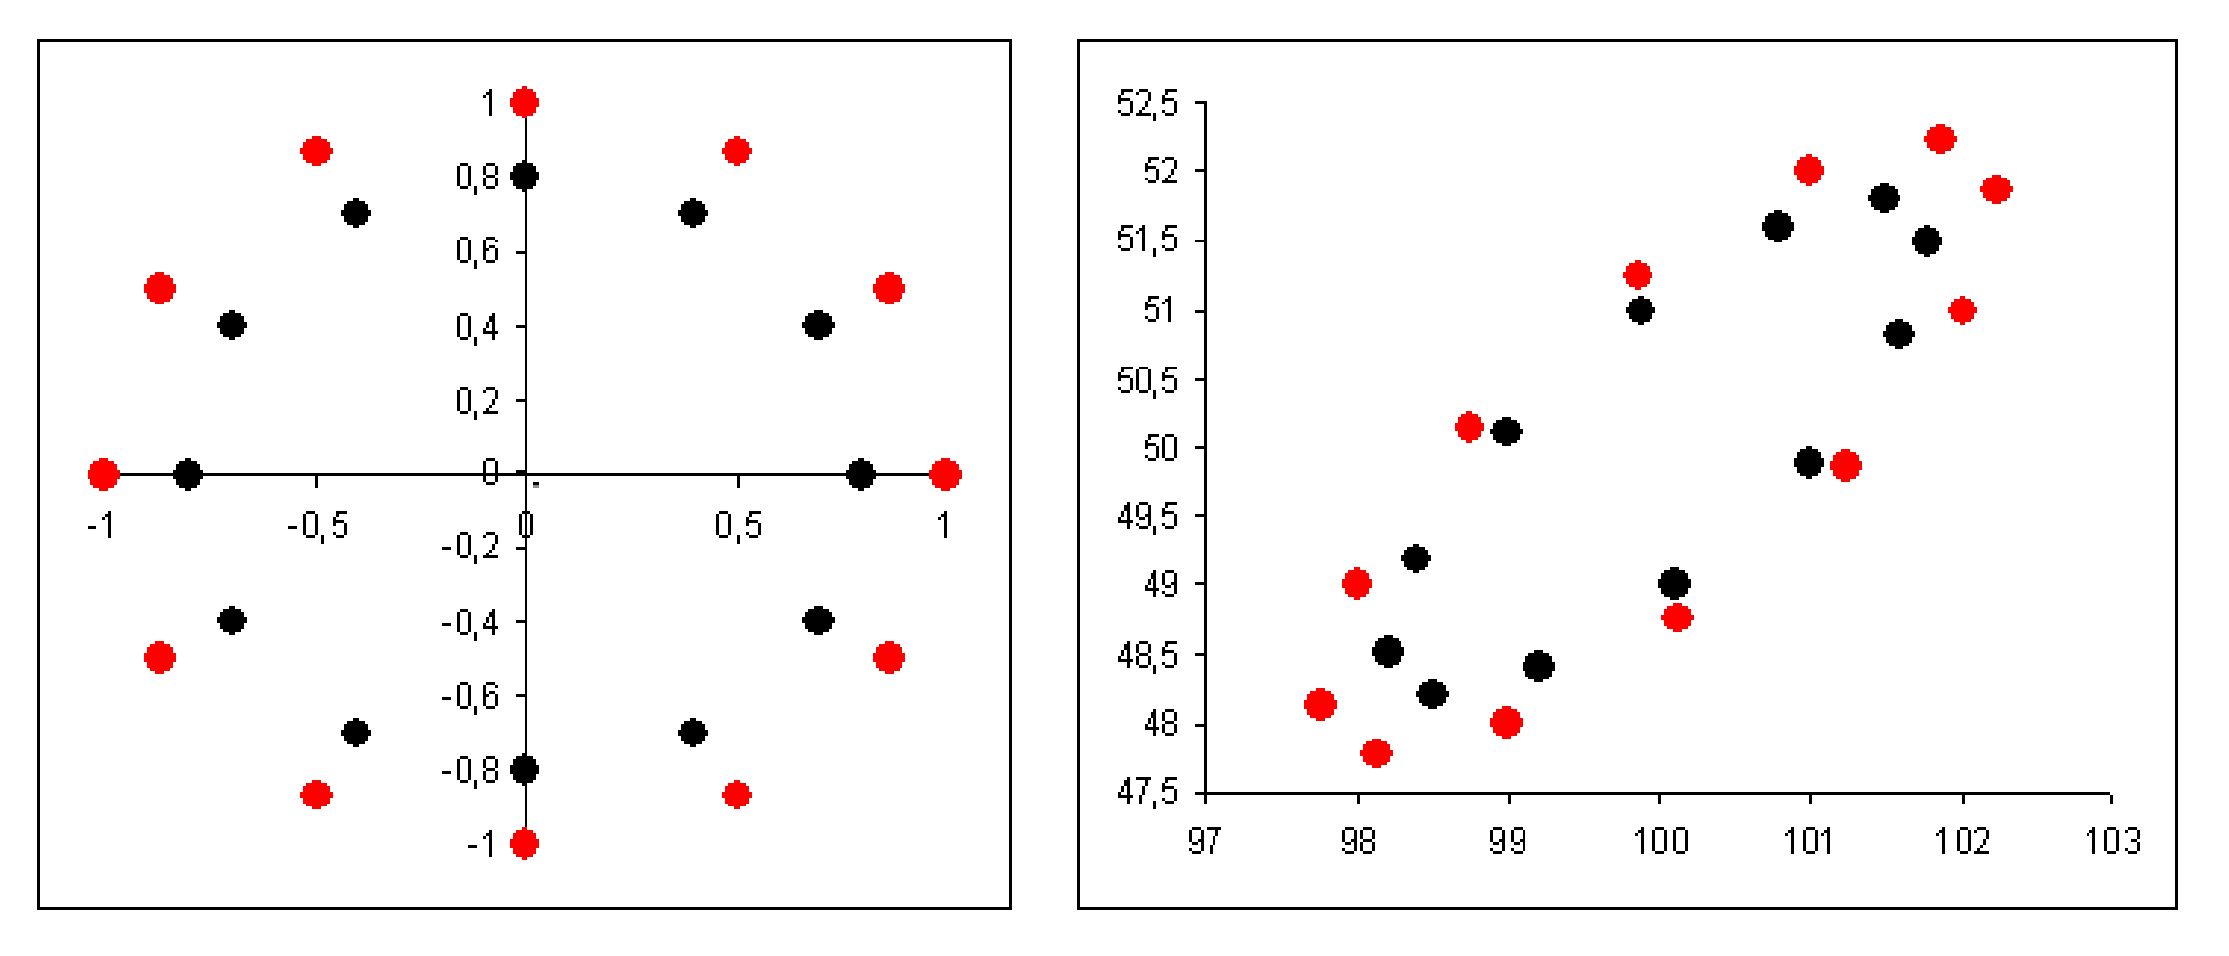
\includegraphics[width=70mm,height=35mm]{img/sdfig7.eps}
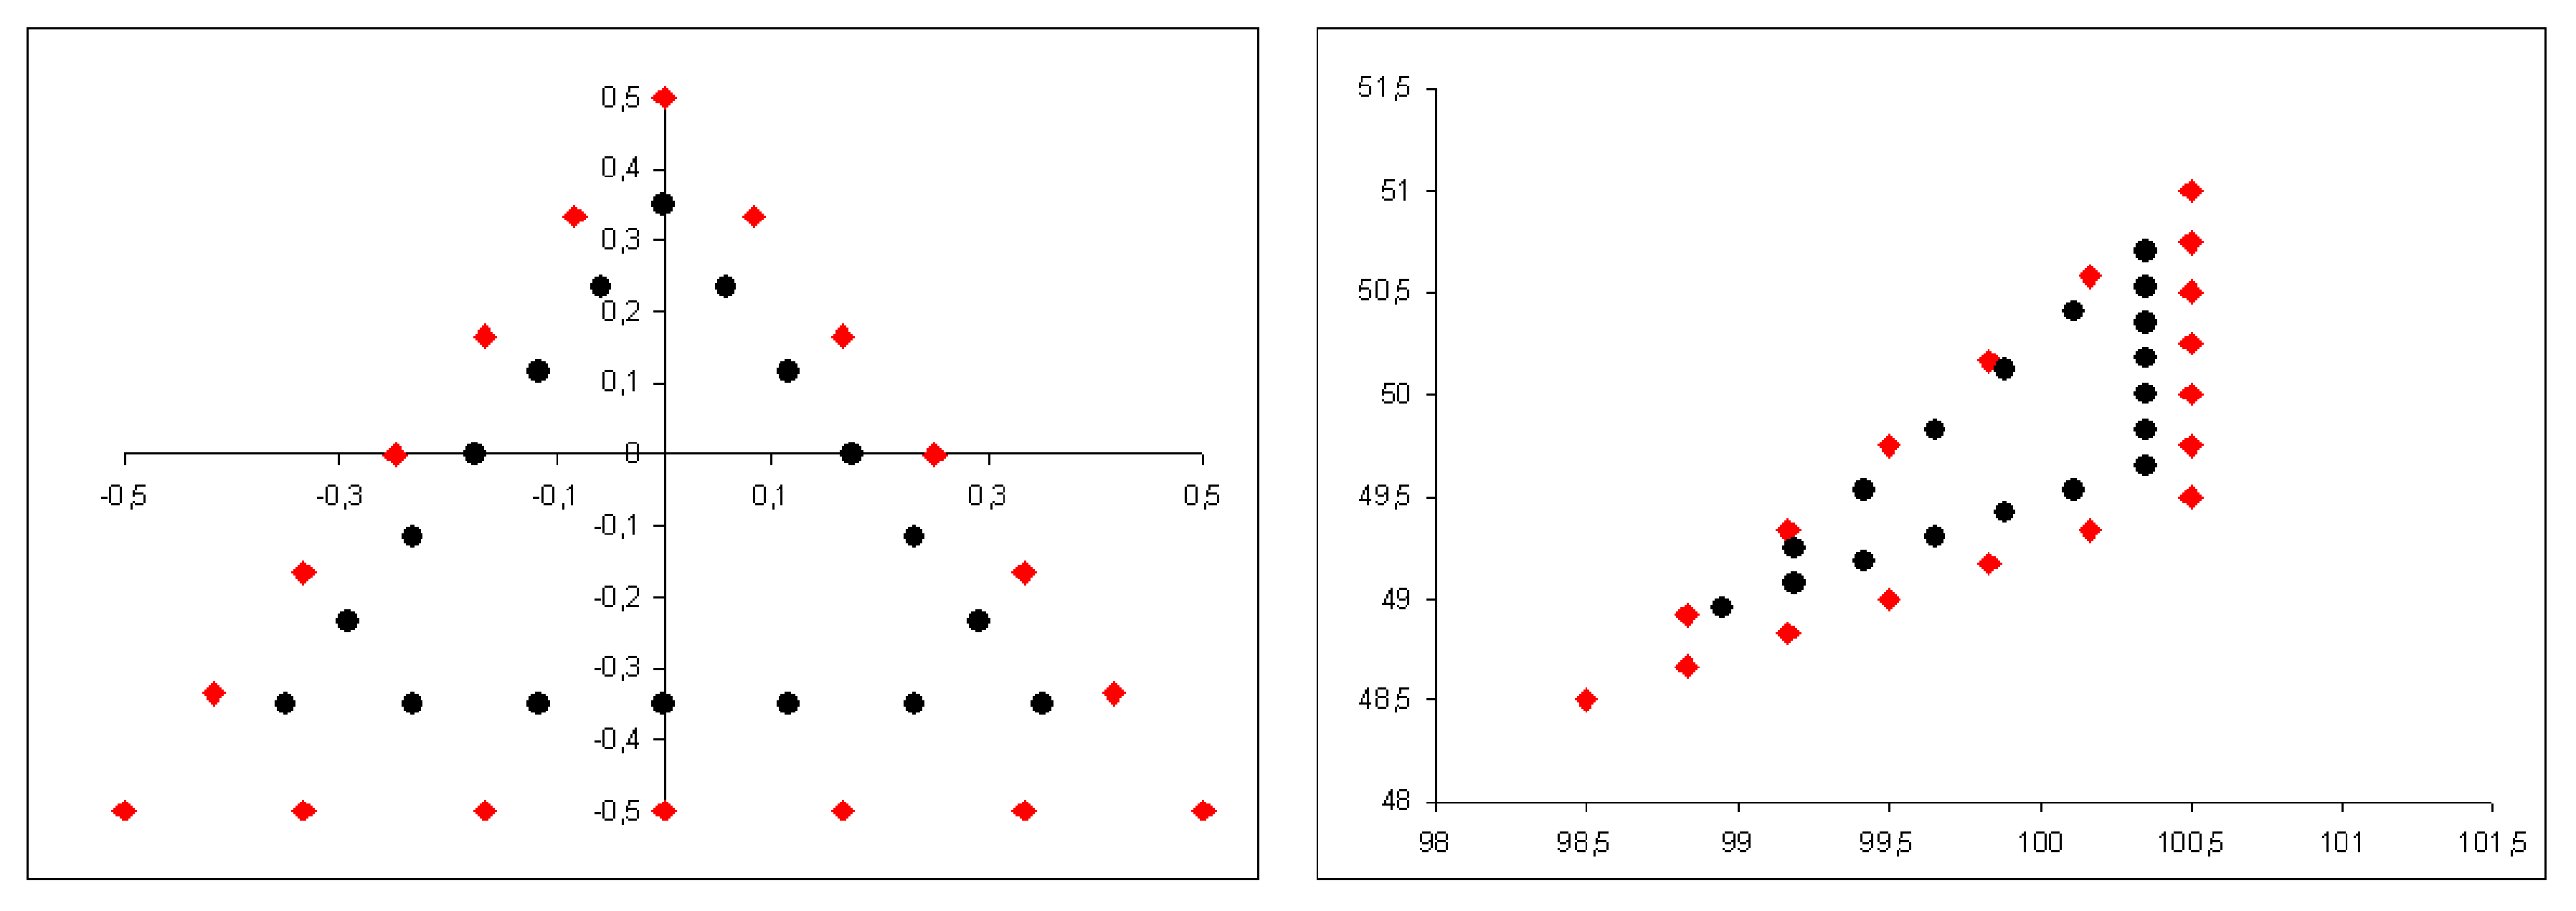
\includegraphics[width=70mm,height=35mm]{img/sdtri1.eps}
\caption{Template characteristic points in (x,y) domain,  and (u,v) domain after geometric transformation for circular and triangular signs.}
\label{fig:sdfig2}
\end{center}
\end{figure}
\par
For complex applications, all of the geometric transformation matrix values can be added to the chromosome encoding in the same manner, however, the resulting search space may not be convenient for real time applications with limited computational power. Therefore, in this application, only the two translation and one scaling coefficients are included in the chromosome in order to reduce the computational requirements. The resulting transition matrix is given in Equation \ref{eq5}.
\begin{eqnarray}
\label{eq5}
\left| \begin{array}{ccc} u \\ v \\ 1 \end{array} \right| &=& 
\left| \begin{array}{ccc} a & 0 & c \\ 0 & a & f \\ 0 & 0 & 1 \end{array} \right| \left| \begin{array}{ccc} x \\ y \\ 1 \end{array} \right|
\end{eqnarray}
\par
The crossover process is also a function of these coefficients as given in Equation \ref{eq6}
\begin{eqnarray}
\label{eq6}
\nonumber a_{newchromo}&=&\alpha.a_{chromo1}+\beta.a_{chromo2} \\
c_{newchromo}&=&\alpha.c_{chromo1}+\beta.c_{chromo2} \\
\nonumber f_{newchromo}&=&\alpha.f_{chromo1}+\beta.f_{chromo2} \\
\nonumber 1&=&\alpha+\beta
\end{eqnarray}
\par
The fitness of the chromosome is evaluated according to the color of the transformed point $(u,v)$ on the binary image. If the value of the pixel is one, which means it is a red point on the original image, the fitness of the chromosome is increased. However, this method fails for completely red regions, therefore another set of template points are introduced in order to indicate the non-red points on the template. These points are also subject to the transformation. These non-red points are selected inside the region bounded by the red points as shown in Figure \ref{fig:sdfig2}. In other words, the red points increase the fitness value when they are white in the binary image, and the black points increase the fitness value when they are black in the binary image. If the expected color cannot be found, then the fitness value is decreased for each of the failed points. At each iteration the fitness values are calculated for each chromosome. At the end of the process the chromosomes are expected to converge around the traffic sign as shown in Figure \ref{fig:sdfig4}.
\begin{figure}[ht]
\begin{center}
\includegraphics[width=60mm,height=35mm]{img/sdfig3.eps}
\includegraphics[width=60mm,height=35mm]{img/sdfig4.eps}
\caption{Initial and converged chromosomes.}
\label{fig:sdfig4}
\end{center}
\end{figure}
\par
After each GA run, half of the converged chromosomes are crossed over to the next frame. This provides the tracking of the detected sings in the video stream.
\subsection{Modified Radial Symmetry}
The initial tests have shown that, GA is likely to find non-existing signs in the regions with relatively high red-color concentration. For preventing false positives, an additional step of \textsl{Modified Radial Symmetry} check is introduced after the GA. 
\par
For circular sign detection, it works as illustrated in Figure \ref{fig:rad_1}. The "Start" point is the outcome of the GA. For each candidate point the GA suggests, the \textit{\textit{Circle Validation algorithm}} detects the innermost circle that surrounds the point. First, the algorithm performs a bi-directional horizontal scan, and finds the x-coordinate center (Center $\sharp$1). The vertical center is detected next, by performing a bi-directional vertical scan starting from Center $\sharp$1. Note that, this is the simplified description of the algorithm. In the actual implementation, the algorithm employs a probabilistic approach, and detects the maximum of 2$^\textit{N}$ x 2$^\textit{N}$ candidate circles, where \textit{N} is the tolerance coefficient. This coefficient helps to tolerate the discontinuities on the circle.
\begin{figure}[ht]
\begin{center}
\includegraphics[scale=0.5]{img/fig_radial1.eps}
\caption{(a) Circle detection, (b) Scoring of circles.}
\label{fig:rad_1}
\end{center}
\end{figure}
\par
After the detection step, each candidate circle is scored as displayed in Figure \ref{fig:rad_1}. The scoring function projects the circle onto the edge-detected image. If the candidate circle really overlaps a circle on the actual image, the candidate gets a high score. The overlapping check is performed for 36 points (10$\degree$ increment) in our implementation. Hence the maximum score is 36.
\begin{figure}[ht]
\begin{center}
\includegraphics[scale=0.5]{img/fig_radial2.eps}
\caption{Candidate circles, and highest score selection}
\label{fig:rad_2}
\end{center}
\end{figure}
\par

\begin{figure}[ht]
\begin{center}
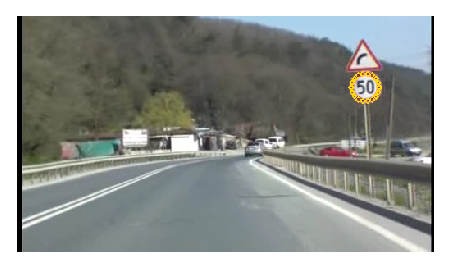
\includegraphics[width=70mm,height=40mm]{img/sdfig5.eps}
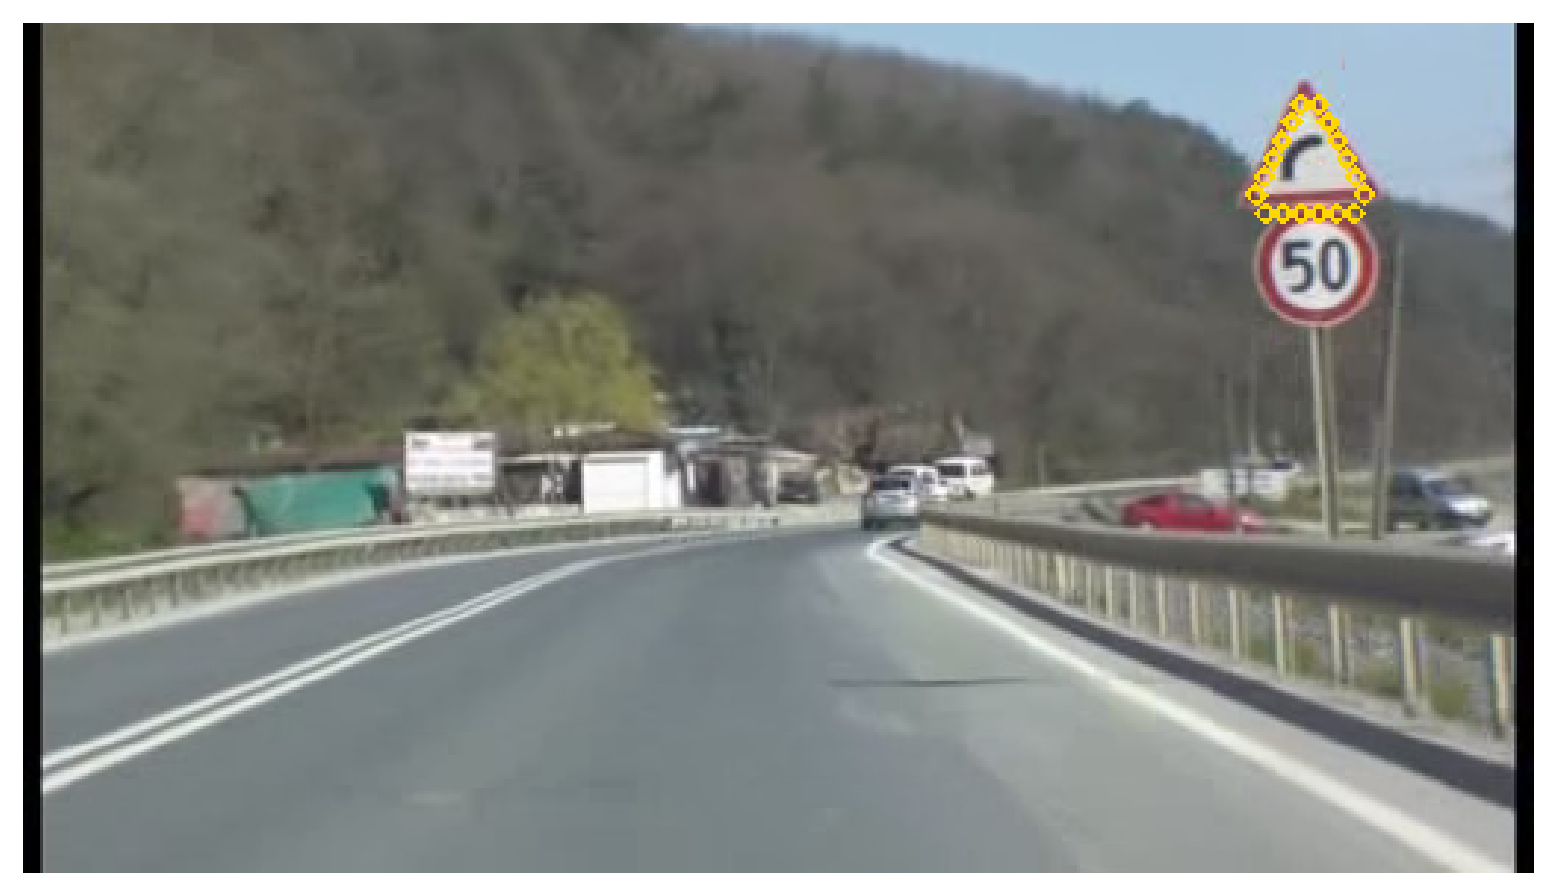
\includegraphics[width=70mm,height=40mm]{img/sdtri2.eps}
\caption{Detected traffic signs.}
\label{fig:sdfig5}
\end{center}
\end{figure}
\par
Triangular sign validation runs in a slightly different manner. As shown in Figure \ref{fig:rad_3}, the detection phase is similar to that of the circular signs, but scoring is completely different. The difference in the geometry affects the Center $\sharp$2 location. Similar to the circle case, the algorithm detects maximum of 2$^\textit{N}$ x 2$^\textit{N}$ candidate triangles, where $\textit{N}$ is the tolerance coefficient. 
\begin{figure}[ht]
\begin{center}
\includegraphics[scale=0.5]{img/fig_radial3.eps}
\caption{Candidate triangles, and highest score selection}
\label{fig:rad_3}
\end{center}
\end{figure}
\par
After the detection step, each candidate triangle is scored as displayed in Figure \ref{fig:rad_2}. The center of the bottom edge is used as the reference point, since it is computationally favorable to deal with right angles. The maximum score a candidate triangle can get is $3 \times 9 = 27$. 

\section{Experiments and Results}
\label{sec:er}
The experiments are performed on a video recorded in a car going with a speed of 60 Km/hour. The video size is 512x288 pixels and frame rate is 20 fps. 

Since the sign detection process should be carried out in real time, we kept the population size and the number of iterations small.  However, in the configuration given below, it is possible to rerun the process several times in a second. This gives an opportunity to utilize the GA to track the detected sign. For this purpose, half of the best chromosomes at the end of each processed frame are crossed over to the next frame. In the proposed implementation, the GA parameters are set as follows;
\begin{itemize}
		\item Population Size: 100
		\item Number of Iterations: 5
		\item Mutation Rate: 0.05
		\item Selection Rate: 0.9
		\item Selection Method: Elitist
\end{itemize}
\par
\begin{figure}[ht]
\begin{center}
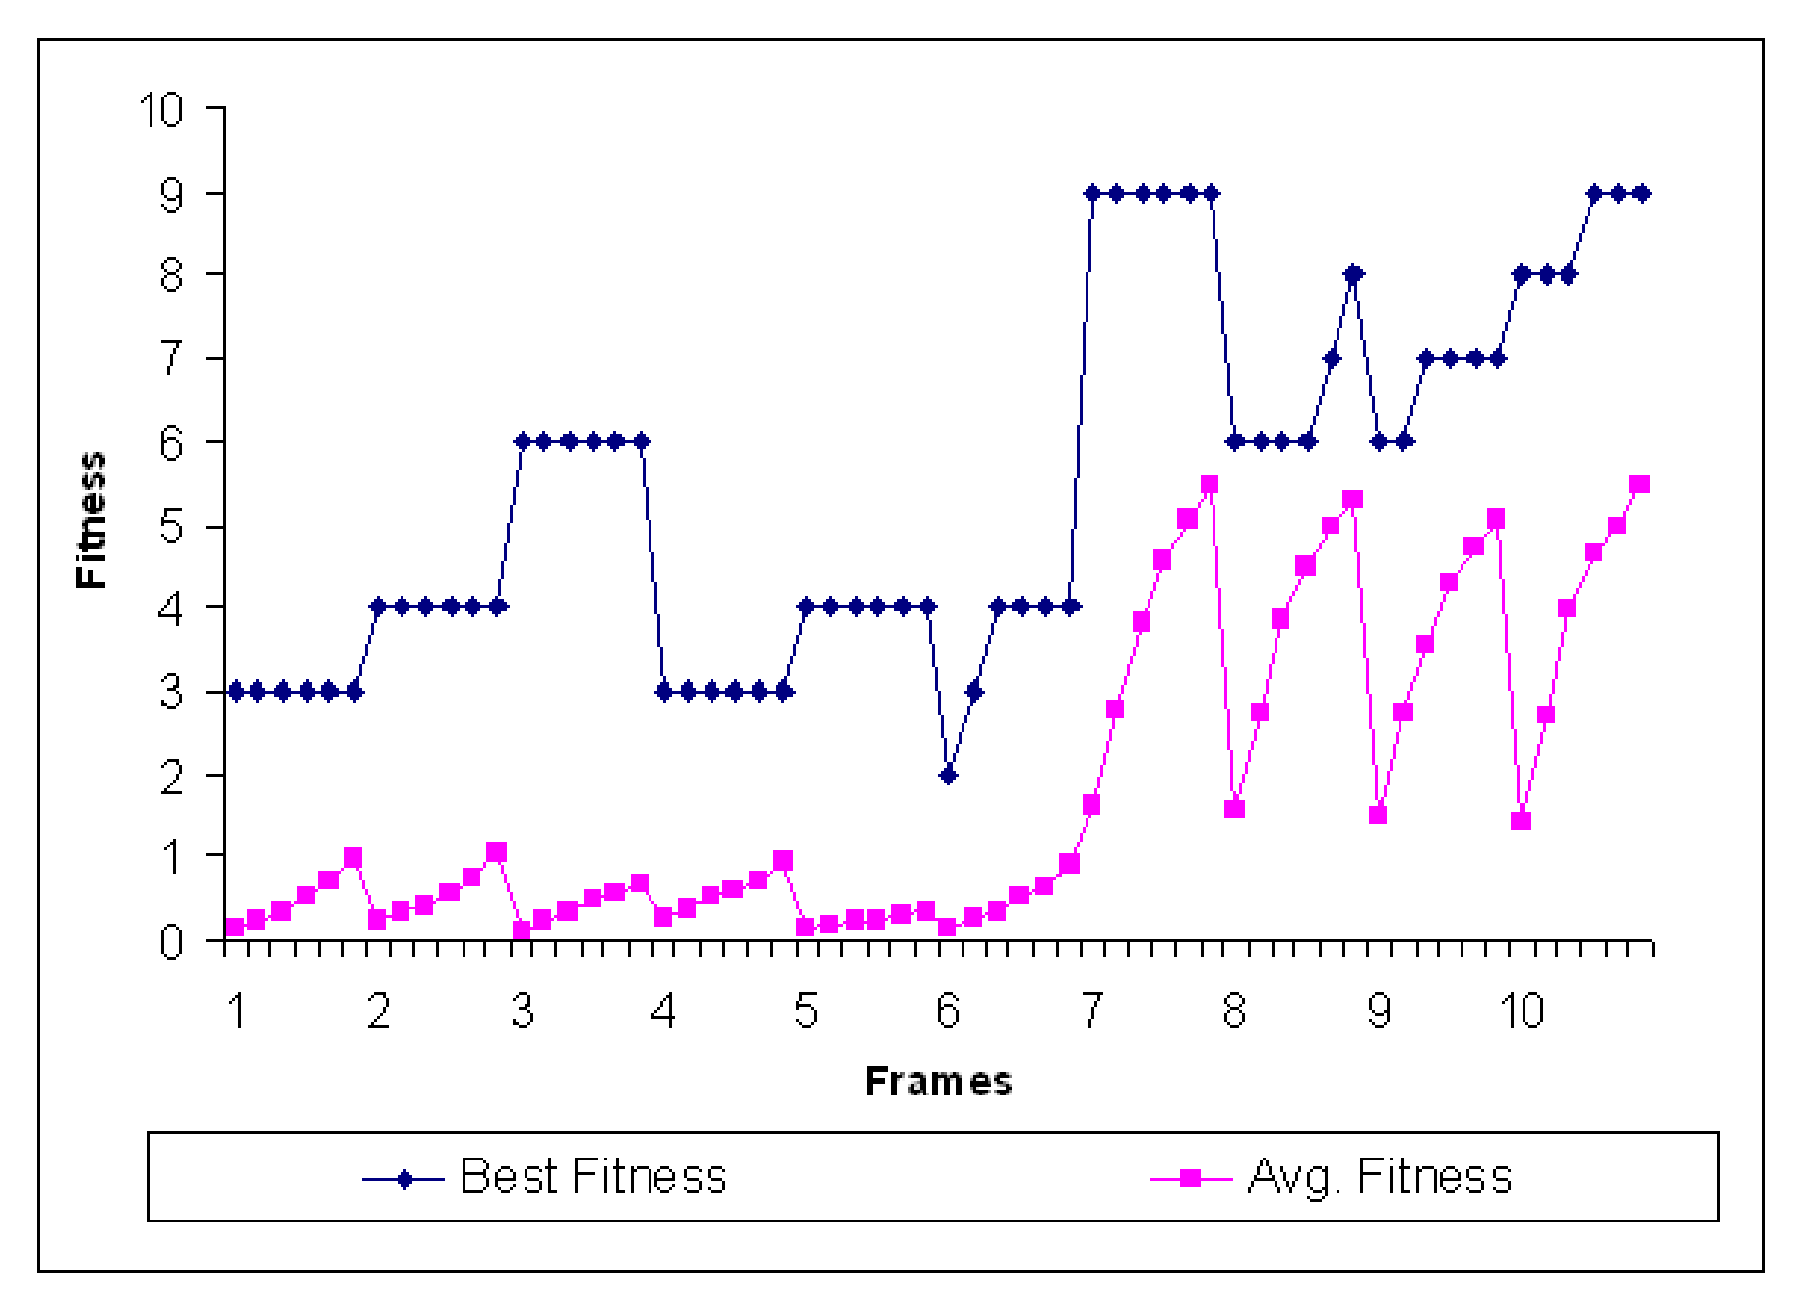
\includegraphics[scale=0.25]{img/gafit.eps}
\caption{The average and best fitness values for 10 frames before detecting the sign.}
\label{fig:gafit}
\end{center}
\end{figure}
\par
The best and average fitness of the population increases significantly when a traffic sign exists in the scene. In Figure \ref{fig:gafit} the change in the fitness values are visualized. In the figure, the average and best fitness values are given for 10 frames which have 5 epochs each. Since half of the population is inherited from previous frame, the best fitness values usually do not decrease when the traffic sign is getting closer.

In \textit{Modified Radial Symmetry} step, we used \textit{N}=2 as the tolerance coefficient. This lets the second level of discontinuity in any of the four directions. The circle or triangle validation took less than 7 milliseconds for each image of the video stream. 
\par
It is generally hard to give exact (success and failure) numbers when dealing with video streams. We have done several measurements and calculated the following results. The complete processing of a single frame takes around 50 milliseconds when it is executed on a laptop PC with Intel T2050 processor at 1.6 GHz. \textit{Radial Symmetry check} has decreased the false alerts rate around $\%$60. 

\section{Conclusion}
This work has proposed a GA approach for the solution of the traffic sign detection and tracking problem. 
The novel contribution is the injection of geometric transformation matrix into GA. This makes the system immune to the rotated and translated signs.  Another contribution is the radial symmetry check for the GA output. This additional step provides the better generations to cross over. 

Although only circular and triangular signs are described in this section, the existing implementation can also process any kind of sign with some constant properties which can be described by a set of characteristic points. 

However, there are certain shortcomings of the proposed method. First of all the image binarization process may suffer from poor lighting conditions and may require additional adaptation processes for special conditions like driving at night and bad weather conditions. Moreover, the proposed approach requires a post-process for classification of the detected signs. The ongoing study for sign classification is intentionally excluded from this paper, since it is entirely another research topic, and definitely employs different methodology. And finally, motion with high speeds ($>$90 Km/hour) should also be tested in realtime.
\bibliographystyle{ieeetr}
\bibliography{SignDetection}	

\end{document}
